%%Capítulo 3 trabajo relacionado 
%
Este capítulo presenta los trabajos relacionados con el tema de esta tesis, se analizan 1) Evaluar el grado de seguridad de un sistema construido usando patrones de seguridad (\textit{Evaluating the degree of security of a system built using security patterns}), 2) Evaluación cuantitativa de la seguridad en arquitecturas de software (\textit{Towards a quantitative assessment of security in software architectures}) y 3) Uso de patrones de seguridad en combinación con métricas de seguridad (\textit{Using security patterns to combine security metrics}).
%
%\vspace{0.3cm}
%
%Cada sección presenta lo propuesto en el trabajo relacionado, donde se describe el problema, los objetivos y la solución a éste. Brevemente se describe la solución propuesta con los resultados obtenidos y por último se presentan las conclusiones del trabajo.

%Evaluating the degree of security of a system built using security patterns
\section{Evaluar el grado de seguridad de un sistema construido usando patrones de seguridad}
%\subsection{Introducción}

Dentro de la variedad de métodos para construir sistemas seguros no se explica cómo evaluar la seguridad de los productos finales. A pesar de que la definición de seguridad no es del todo clara para los sistemas de información, existen pocas métricas aceptadas pero que son complicadas de aplicar. El artículo \textit{``Evaluating the degree of security of a system built using security patterns''} \cite{FerYosWas18} propone una métrica utilizando una aproximación  de búsqueda de amenazas en sistemas que han sido construido utilizando patrones. 

\vspace{0.3 cm}

Tomando como definición de la seguridad de sistemas como la habilidad de proteger a los activos ante ataques internos o externos, el método define un listado de amenazas y verifica cuales amenazas están siendo mitigadas por al menos un patrón de seguridad. La métrica consiste en la cantidad de amenazas que están atendidas por un patrón de seguridad. 

\vspace{0.3 cm}

Una amenaza $T_i$ usa una secuencia de pasos de ataque $T_{ik}$, es decir, $T_i \rightarrow T_{i1},T_{i2},...,T_{ij}$, para detener $T_i$ es suficiente con detener alguna de los  $T_{ij}$. Los patrones de seguridad describen qué ataques pueden detener, dado que el método propuesto por \cite{FerYosWas18} contempla que el sistema ha sido previamente construido con patrones de seguridad, se sabe que hay un conjunto de pasos de ataque que están siendo mitigados. Contabilizando el número de amenazas mitigadas $TN$ y conociendo el número total de amenazas identificadas $T$, la métrica de seguridad SC se define como $SC=\frac{TN}{T}$.

\vspace{0.3 cm}

El proceso para evaluar la seguridad de un sistema consiste en:

\begin{itemize}[noitemsep]
	\item Enumerar las amenazas basándose en las metas del atacante (parte de la metodología de desarrollo).
	\item Elegir las amenazas de acuerdo a probabilidad o impacto de ocurrencia. 
	\item Determinar SC con todas o las amenazas más importantes.
\end{itemize}

La obtención de las amenazas del sistema se deriva durante las etapas de obtención de requisitos y diseño del desarrollo de software, donde se analiza cada actividad dentro del diagrama de actividades de un caso de uso, observando cómo podría un atacante cumplir sus metas. 

\vspace{0.3 cm}

Se propone una manera de refinar la métrica SC utilizando la aproximación \textit{Twin peaks}, que se refiere a una forma iterativa de construir arquitecturas de software. El método de enumeración de amenazas comienza por un modelo de seguridad conceptual donde los patrones de seguridad han sido agregados al modelo funcional (obtenido de los requisitos funcionales del sistema), entonces se analiza cada caso de uso para generar el diagrama de actividades que es el que revela las amenazas como metas del atacante e identifica los activos a proteger. 

\vspace{0.3 cm}

Utilizando \textit{Twin peaks} se produce una nueva arquitectura en cada ciclo, es decir, cada ciclo contempla los mismos casos de uso pero a mayor detalle considerando nuevos elementos como se muestra en la Figura \ref{fig:twinpeaks}.

\begin{figure}[!h]
  \centering
    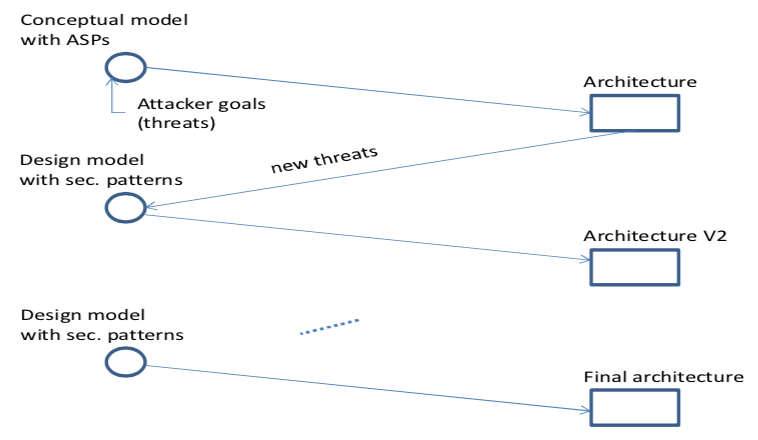
\includegraphics[scale=0.5]{Imagenes/fig_iteTwinPeaks.png}
    \caption{Iteraciones \textit{Twin peaks} obtenida de \cite{FerYosWas18}.}
    \label{fig:twinpeaks}
\end{figure}

La métrica propuesta realiza la enumeración de las amenazas como parte de la metodología de desarrollo del software donde cada ataque es descrito como un patrón de mal uso, pero no hay forma de mostrar que todos los patrones de mal uso relevantes para el sistema han sido considerados. Una ventaja es que, al identificar los patrones de seguridad aplicados al sistema se identifica a un gran número de patrones de mal uso mitigados. 

\vspace{0.3 cm}

La métrica presentada utiliza un método de enumeración de amenazas específico, no obstante puede aplicarse a sistemas que tengan una enumeración de amenazas obtenidas de métodos diferentes. Cabe resaltar que la enumeración solo contempla cierto número de amenazas dentro de las etapas del ciclo de vida del desarrollo del sistema o en las iteraciones de \textit{Twin Peaks}.

%% Measuring the level of security introduced by security patterns - Eduardo B. Fernandez - 2010
%\section{Metodología para evaluar el nivel de seguridad de un sistema implementando patrones de seguridad}
%%Problema - Solución - Procedimiento - Resultados - Contribuciones 
%
%%\subsection{Introducción}
%%
%Se han buscado formas de evaluar la implementación de patrones de seguridad para mejorar la seguridad en los sistemas, muchos autores se enfocan a la evaluación individual de los patrones y no como un todo, por esto en el artículo \textit{``Measuring the level of security introduced by security pattern''} \cite{Was10} la pregunta abordada es ¿qué grado de seguridad alcanza un sistema usando los patrones de seguridad en su construcción? y la solución propuesta es una metodología para construir sistemas seguros a través del uso de patrones de seguridad  y su evaluación sobre los posibles ataques definidos como patrones de mal uso. 
%
%\vspace{0.3 cm}
%
%La metodología consiste en una comparación de dos sistemas construidos bajo los mismos requisitos, con la diferencia que uno de ellos implementa patrones de seguridad en el diseño y el otro no. Se consideran las amenazas que pueden sufrir los sistemas y son asociadas a un determinado patrón de mal uso. Entonces, para realizar la evaluación, ambos sistemas son sometidos a la misma cantidad de amenazas y se observa cuántas de ellas consiguen ser mitigadas por cada sistema. El conjunto de relaciones entre amenazas mitigadas por patrones de seguridad son comparadas entre los sistemas. Este valor indica qué tan seguro es el software. 

%\subsection{Descripción de la metodología}
%
%\begin{enumerate}[noitemsep]
%	\item \textbf{Identificación de amenazas del sistema}. Esta metodología se basa en que existen requisitos previos, entonces, tomando esos requisitos se buscan las posibles amenazas que pudieran afectar al sistema una vez construido. Una vez identificadas, se procede a la elección de Patrones de mal uso que las definan. 
%	\item \textbf{Elección de Patrones de mal uso}. Las amenazas a un sistema pueden expresarse como Patrones de mal uso que son una forma de proyectar la amenaza de acuerdo a su objetivo. Existen más de un Patrón de mal uso para realizar cierto tipo de ataques, por lo que los autores asociaron una cantidad de éstos patrones a un tipo de amenaza para la metodología. 
%	\item \textbf{Elección de patrones de seguridad}. Dado que los patrones de seguridad proveen soluciones ante una amenaza específica, los autores utilizaron la asociación amenaza-patrones de mal uso anterior para relacionar a los patrones directamente con la amenaza de seguridad que estos mitigan y su grupo de Patrones de mal uso.  
%	\item \textbf{Evaluación de los sistemas}. Para la evaluación, la metodología propone la construcción de dos sistemas bajo los mismos requisitos, uno de los sistemas es diseñado con patrones de seguridad y el otro sin ellos. Entonces, se realiza la comparación de los sistemas enumerando el conjunto de amenazas mitigadas por cada sistema. La aplicación de la metodología permite una estimación de la seguridad que están adicionando los patrones de seguridad. 
%\end{enumerate}
%
%Como se puede apreciar en la Figura \ref{diagrama-tr1}, ambos sistemas son sometidos a la misma cantidad y tipo de amenazas, por lo que el resultado arrojado de la evaluación da un parámetro que indica el nivel de seguridad que otorga un conjunto de patrones de seguridad a un sistema. Una ventaja de esta metodología es que realiza una evaluación de un sistema completo y no solo de un Patrón de Seguridad desde la fase de diseño. Cabe resaltar que la evaluación no determina si los patrones de seguridad son implementados correctamente, para ello se requiere pasar a la fase de pruebas. 
%
%\begin{figure}[!tbp]
%  \centering
%    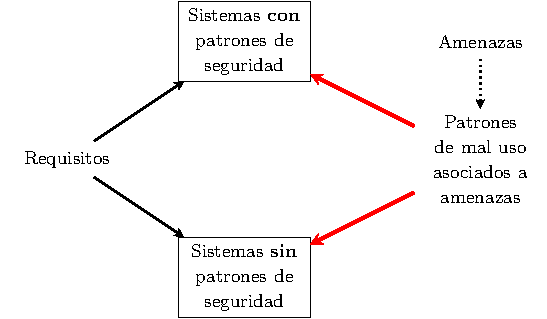
\includegraphics[scale=1]{Imagenes/diagrama3_1.eps}
%    \caption{Diagrama de comparación de sistemas.}
%    \label{diagrama-tr1}
%\end{figure}
%
%\subsection{Conclusiones del trabajo}
%Un sistema de software que ha sido diseñado utilizando los patrones de seguridad es capaz de detener cada amenaza esperada y se puede considerar al sistema seguro a un nivel de modelado. Además, este trabajo plantea definir de manera más precisa la relación entre los patrones de mal uso y las metas de los atacantes para mejorar el análisis del sistema como un todo. 
%
%\subsection{Semejanzas}
%\begin{itemize}[noitemsep]
%	\item Busca identificar si los patrones de seguridad proporcionan un nivel de seguridad a un sistema
%	\item Realiza la evaluación de un sistema completo
%	\item Evalúa un conjunto de patrones de seguridad 
%	\item Desde la fase de diseño se realiza una estimación de la cantidad de seguridad agregada al utilizar patrones de seguridad
%\end{itemize}
%\subsection{Diferencias}
%\begin{itemize}[noitemsep]
%	\item Propone una metodología y no una métrica
%	\item La comparación se realiza una vez construidos los sistemas 
%	\item Se enfoca en la relación que existe entre los patrones de seguridad y los Patrones de mal uso
%\end{itemize}
%
%%------------------------------------------------
%%Towards a quantitative assessment of security in software architectures - Artsiom Yautsiukhin - 
%
\section{Evaluación cuantitativa de la seguridad en arquitecturas de software}
%%Problema - Solución - Procedimiento - Resultados - Contribuciones 
%
%\subsection{Introducción}
%
%La literatura que se encuentra sobre evaluación de la seguridad se enfocan a medir la seguridad después de haber desarrollado un sistema y debido a que actualmente los sistemas son más grandes y heterogéneos, la evaluación después de construido el sistema se convierte en algo más complejo. 

En el artículo \textit{``Towards a quantitative assessment of security in software architectures''} \cite{YauScaHey} propone una aproximación para evaluar la seguridad en arquitecturas de software basadas en patrones. En particular, los patrones de seguridad se utilizan para medir que extensión de una arquitectura está protegida con respecto a las amenazas de seguridad más relevantes. 

\vspace{0.3cm}

Esta metodología se divide en 4 partes \cite{YauScaHey}:

\begin{enumerate}[noitemsep]
	\item \textbf{Mapeo de amenazas con los objetivos de seguridad}. Haciendo uso de la metodología STRIDE de Microsoft, se seleccionan las amenazas que estén relacionadas con el modelado del software. Cada amenaza es organizada en árboles de amenaza y descompuesto a lo más en tres niveles.
	\item \textbf{Clasificación de las amenazas de acuerdo a su severidad}. Dado que cada amenaza tiene un grado de severidad diferente, se recurre a una clasificación otorgándoles pesos a cada amenaza para diferenciarlos. Cada peso está determinado por el nivel de riesgo definido en la DREAD de Microsoft. 
	\item \textbf{Determinación de la protección ante una amenaza}. Para determinar el nivel de protección que otorga un patrón de seguridad ante una amenaza, se asocian las amenazas a los objetivos de seguridad a los que el patrón contribuye. 
	\item \textbf{Cálculo de la cobertura de seguridad}. El cálculo se realiza por rama en el árbol de amenazas. Las hojas del árbol representarán el valor de protección que otorgan los patrones de seguridad para un requisito
\end{enumerate}

A cada arista del árbol de requerimientos se le asignan pesos, estos pesos reflejan el impacto a cada requisito de manera individual calificando la pérdida monetaria si es que el requisito de seguridad falla.

\vspace{0.3cm}

La parte experimental consiste en realizar dos sistemas utilizando el mismo conjunto de requisitos pero con una estrategia diferente para la selección de los patrones de seguridad en cada sistema. El primero se enfocó en seleccionar un conjunto de patrones de seguridad que cubriera lo mínimo pero suficiente los requisitos y el segundo se enfocó en proporcionar la mejor solución de seguridad sin importar el costo de implementación. La Figura \ref{fig:reqTree} muestra la descomposición de los objetivos con patrones del ejemplo utilizado en este artículo.

\begin{figure}[!h]
  \centering
    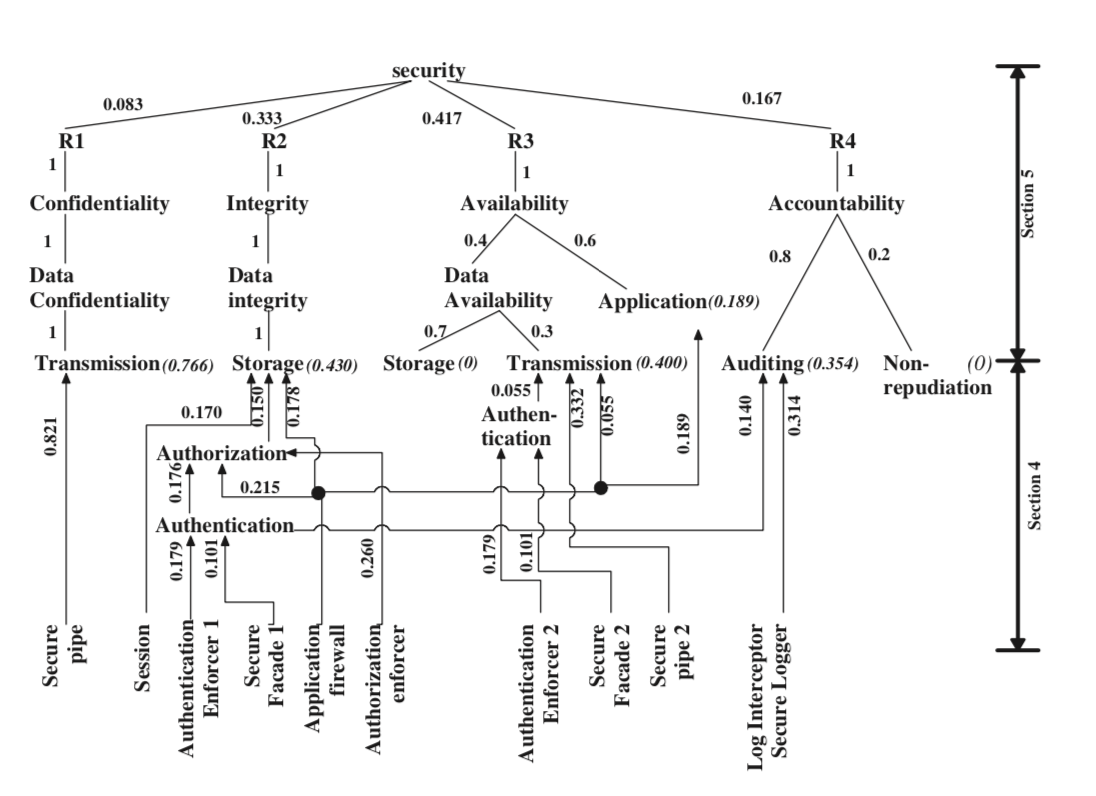
\includegraphics[scale=0.45]{Imagenes/fig_reqTree.png}
    \caption{Descomposición de objetivos con patrones obtenida de \cite{YauScaHey}.}
    \label{fig:reqTree}
\end{figure}

\vspace{0.3cm}

La metodología propuesta es aplicada a un alto nivel de abstracción del diseño de software para encontrar posibles errores lo más rápido posible. Tanto el uso de árboles de objetivos de seguridad y amenazas dan un panorama debido a que las amenazas están en constante cambio. Se hace un énfasis en los niveles de seguridad para los requerimientos, ya que fueron asignados de manera empírica por la experiencia de los autores, además de utilizar STRIDE como el conjunto de amenazas base de la evaluación. 


%
%\subsection{Semejanzas }
%Este trabajo relacionado se asemeja en el presente trabajo de tesis en:
%
%\begin{itemize}[noitemsep]
%	\item Hace una evaluación cuantitativa
%	\item Utiliza metodologías probadas para relacionar los requisitos de seguridad con los patrones de seguridad (STRIDE)
%	\item Marca una secuencia para la definición de los patrones
%\end{itemize}
%
%\subsection{Diferencias}
%\begin{itemize}[noitemsep]
%	\item No utiliza la métrica directamente en la evaluación del patrón de seguridad
%	\item Requiere la evaluación de un experto para elegir el peso de las amenazas
%\end{itemize}
%
%%------------------------------------------------
%% Using security patterns to combine security metrics - Thomas Heyman - 
\section{Uso de patrones de seguridad en combinación con métricas de seguridad}
%
%%Problema - Solución - Procedimiento - Resultados - Contribuciones 
%
%\subsection{Introducción}
%
Uno de los problemas analizados en la evaluación de los patrones de seguridad es la correcta selección de métricas para la medición de seguridad y su interpretación. En el artículo titulado \textit{``Using security patterns to combine security metrics''} \cite{HeyScaHuy08}, se propone un método que al evaluar la correcta selección de los patrones de seguridad sobre un sistema se obtiene un indicador de si estos consiguen atender un objetivo de seguridad. 
%
%\subsection{Descripción de la metodología}
La metodología consiste en 3 pasos \cite{HeyScaHuy08}:
%
\begin{enumerate}[noitemsep]
	\item \textbf{Definición de patrones de seguridad a partir de los objetivos}. Esta metodología considera que existen requisitos de seguridad, los cuales deben ser extrapolados a uno o más objetivos de seguridad. Un vez que se tienen especificados los objetivos, se buscan los patrones de seguridad que contribuirán al cumplimiento de cada objetivo. 
	\item \textbf{Selección de métricas}. El proceso de selección de métricas va implícito en la selección del Patrón de Seguridad. Cabe resaltar que los resultados de las métricas son relevantes para los objetivos de seguridad. Los autores proponen el uso de gráficas de dependencias, las cuales facilitan la selección de métricas y dichas gráficas son construidas en la etapa de diseño. Para cada requerimiento de seguridad se define una gráfica de dependencia. Cada gráfica consiste en tres capas:
\begin{itemize}[noitemsep]
	\item Objetivos de alto nivel. Aquí se identifica la relación entre diferentes objetivos de seguridad. 
	\item Objetivo de seguridad resuelto por un patrón. Uno o más patrones de seguridad pueden colaborar para resolver un objetivo de seguridad. En esta capa, se describe si existe esa relación o no. 
	\item Métricas de patrones de seguridad. En esta última capa, son agregadas las métricas a los patrones que se están evaluando.
\end{itemize}
	\item \textbf{Interpretación de resultados}. Los resultados obtenidos de las métricas son interpretados en el contexto del patrón de seguridad a los que están asociados. Con ellos se comprueba si el Patrón de Seguridad está siendo correctamente implementado. Si un resultado no es el deseado, se puede recurrir a la gráfica de dependencia para localizar qué patrón de seguridad no está siendo bien aplicado y corregirlo. Un ejemplo de una gráfica de dependencias se muestra en la Figura \ref{diagrama-tr2}, donde a los patrones de seguridad son relacionados con las métricas correspondientes; también se tiene que más de un patrón pueden resolver una característica de seguridad como \textit{Audit Interceptor} y \textit{Secure Logger} a la Auditoría.
\end{enumerate}
%
\begin{figure}[!hp]
  \centering
    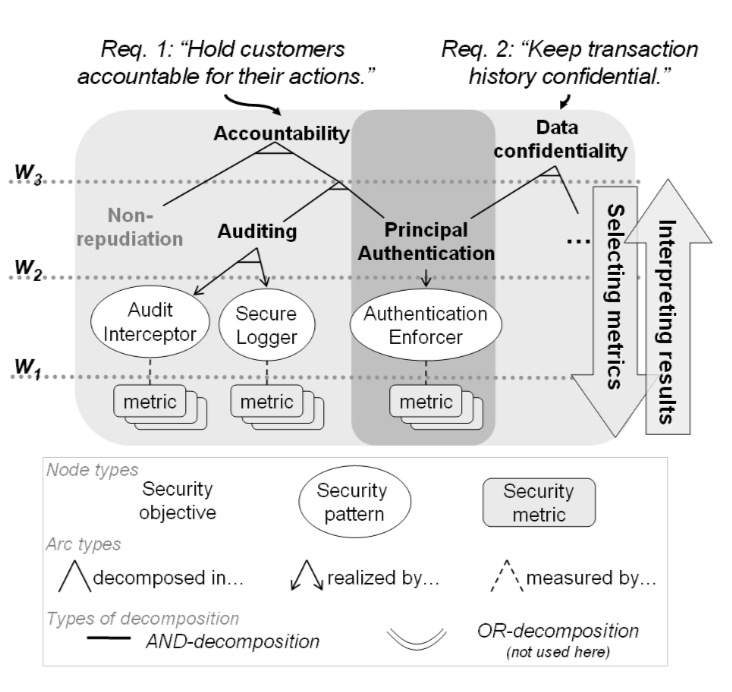
\includegraphics[scale=0.45]{Imagenes/fig_depGraph.png}
    \caption{Gráfica de dependencias obtenida de \cite{HeyScaHuy08}.}
    \label{diagrama-tr2}
\end{figure}
%
%\subsection{Conclusiones del trabajo}
%
La solución en este trabajo pretende hacer una integración fácil de las métricas y su asociación con los patrones de seguridad, dicha asociación permite obtener un estado del nivel de seguridad del sistema a través de sus objetivos de seguridad. En particular, la solución toma en cuenta las métricas sobre lo que debería hacer el sistema sin tratar de detectar ataques específicos. 
%
%\subsection{Semejanzas }
%Este trabajo relacionado se asemeja en el presente trabajo de tesis en:
%
%\begin{itemize}[noitemsep]
%	\item Se basan en patrones de seguridad para determinar el nivel de seguridad de un sistema
%	\item Usa métricas para determinar el correcto funcionamiento de un Patrón de Seguridad
%	\item Hace el análisis en la fase de diseño
%\end{itemize}
%
%\subsection{Diferencias}
%\begin{itemize}[noitemsep]
%	\item Utiliza métricas ya establecidas por cada Patrón de Seguridad y evalúa cada uno.
%	\item La metodología sirve para identificar si hay posibles errores en los patrones de seguridad e identificar que objetivo de seguridad es el que no se está cumpliendo.
%\end{itemize}
%
%
%
\section{Resumen}

En este capítulo se presenta el resumen de tres trabajos relacionados con la evaluación de los patrones de seguridad. El primer trabajo presenta una métrica de seguridad denominada SC la cual contabiliza el total de amenazas mitigadas por patrones de seguridad entre el total de amenazas. Una de las mejoras que propone es utilizar la aproximación \textit{Twin peaks} que produce una nueva arquitectura en cada ciclo contemplando los mismos casos de uso pero a mayor detalle.

\vspace{0.3cm}

El segundo trabajo presenta una metodología que consiste en medir qué extensión de una arquitectura está protegida con respecto a las amenazas de seguridad más relevantes. La metodología consiste en cuatro partes: 1) mapeo de las amenazas con los objetivos de seguridad, 2) clasificación de las amenazas de acuerdo a su severidad, 3) determinación de la protección ante una amenaza y 4) cálculo de la cobertura de seguridad. 

\vspace{0.3cm}

Por último, el tercer trabajo presenta una metodología que permite elegir los patrones de seguridad con respecto a los objetivos de seguridad y las métricas que evaluarán a los patrones. La metodología se divide en tres fases que son: 1) definición de los patrones de seguridad a partir de los objetivos de seguridad, 2) selección de métricas e 3) interpretación de resultados. Este trabajo tiene como objetivo integrar las métricas a la evaluación de un sistema que está utilizando los patrones de seguridad. 